% Shared TikZ styles and layouts for the paper-style system architecture.
% The three layouts below intentionally use the same implementation semantics.

\definecolor{archtext}{gray}{0.12}
\definecolor{archline}{gray}{0.22}
\definecolor{archmuted}{gray}{0.42}
\definecolor{archfill}{gray}{0.975}
\definecolor{archgroup}{gray}{0.48}
\definecolor{archmeasure}{gray}{0.34}

% Keep the disturbance accent muted and reproducible.
\colorlet{archpush}{orange!78!black}

\tikzset{
  >=stealth,
  archblock/.style={
    rectangle,
    draw=archline,
    fill=archfill,
    line width=0.72pt,
    align=center,
    inner xsep=1.8mm,
    inner ysep=1.25mm,
    minimum height=11.5mm,
    font=\scriptsize,
    text=archtext,
  },
  archref/.style={archblock, text width=28mm},
  archtask/.style={archblock, text width=33mm},
  archqp/.style={archblock, text width=39mm},
  archplant/.style={archblock, text width=35mm},
  archeval/.style={archblock, text width=40mm},
  archsignal/.style={
    ->,
    draw=archline,
    line width=0.66pt,
    shorten <=0.5pt,
    shorten >=0.5pt,
  },
  archfeedback/.style={archsignal, draw=archline},
  archmeasurement/.style={archsignal, draw=archmeasure},
  archpushsignal/.style={
    archsignal,
    draw=archpush,
    dashed,
  },
  archlabel/.style={
    font=\scriptsize,
    text=archtext,
    fill=white,
    inner sep=0.75pt,
    align=center,
  },
  archmathlabel/.style={
    font=\scriptsize,
    text=archtext,
    fill=white,
    inner sep=0.75pt,
    align=center,
  },
  archpushlabel/.style={archlabel, text=archpush},
  archmeasurelabel/.style={archlabel, text=archmeasure},
  archboundary/.style={
    draw=archgroup,
    dashed,
    line width=0.58pt,
  },
  archboundarylabel/.style={
    font=\scriptsize,
    text=archgroup,
    fill=white,
    inner sep=1pt,
  },
  archinput/.style={
    font=\scriptsize,
    text=archtext,
    align=right,
    inner sep=0pt,
  },
}

% Candidate A: a conventional horizontal controls loop.  The controller
% boundary is deliberately quiet; the signal topology does most of the work.
\newcommand{\DrawArchitectureCandidateA}{%
  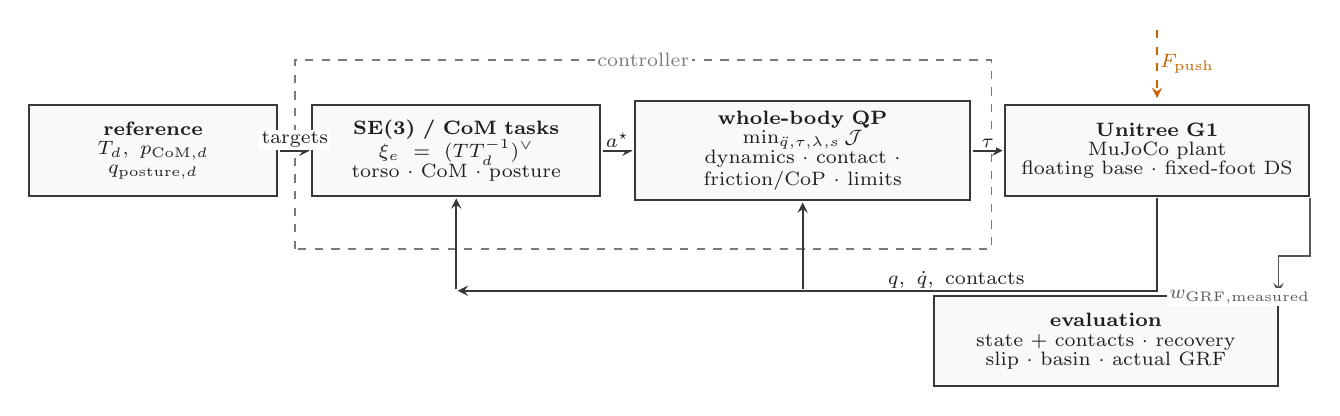
\begin{tikzpicture}[x=1cm,y=1cm]
    \ifdefined\CandidateSheet
      \node[anchor=west,font=\scriptsize,text=archmuted] at (-0.05,4.45)
        {Candidate A - classical horizontal closed loop};
    \fi

    % Controller boundary excludes the plant and the evaluation block.
    \draw[archboundary] (3.35,1.45) rectangle (12.20,3.85);
    \node[archboundarylabel] at (7.775,3.85) {controller};

    \node[archref] (aref) at (1.55,2.70) {\textbf{reference}\\[-1pt]
      {\scriptsize $T_d,\ p_{\mathrm{CoM},d}$}\\[-1pt]
      {\scriptsize $q_{\mathrm{posture},d}$}};
    \node[archtask] (atask) at (5.40,2.70) {\textbf{SE(3) / CoM tasks}\\[-1pt]
      $\xi_e=\Log(TT_d^{-1})^\vee$\\[-1pt]
      {\scriptsize torso $\cdot$ CoM $\cdot$ posture}};
    \node[archqp] (aqp) at (9.80,2.70) {\textbf{whole-body QP}\\[-1pt]
      $\min_{\ddot q,\tau,\lambda,s}\mathcal{J}$\\[-1pt]
      {\scriptsize dynamics $\cdot$ contact $\cdot$ friction/CoP $\cdot$ limits}};
    \node[archplant] (aplant) at (14.30,2.70) {\textbf{Unitree G1}\\[-1pt]
      MuJoCo plant\\[-1pt]
      {\scriptsize floating base $\cdot$ fixed-foot DS}};
    \node[archeval] (aeval) at (13.65,0.28) {\textbf{evaluation}\\[-1pt]
      {\scriptsize state + contacts $\cdot$ recovery}\\[-1pt]
      {\scriptsize slip $\cdot$ basin $\cdot$ actual GRF}};

    \draw[archsignal] (aref.east) --
      node[archlabel,above] {targets}
      (atask.west);
    \draw[archsignal] (atask.east) -- node[archmathlabel,above] {$a^\star$} (aqp.west);
    \draw[archsignal] (aqp.east) -- node[archmathlabel,above] {$\tau$} (aplant.west);

    % External disturbance bypasses the dashed controller boundary.
    \draw[archpushsignal] (14.30,4.25) --
      node[archpushlabel,right] {$F_{\mathrm{push}}$} (14.30,3.35);

    % Plant state returns to both controller blocks through a shared bus.
    \coordinate (afb) at (14.30,0.92);
    \draw[archfeedback] (aplant.south) -- (afb) -- (5.40,0.92);
    \draw[archfeedback] (5.40,0.92) -- (atask.south);
    \draw[archfeedback] (9.80,0.92) -- (aqp.south);
    \node[archlabel,above] at (11.75,0.92) {$q,\ \dot q,\ \mathrm{contacts}$};

    % A separate physical-measurement path keeps measured GRF distinct from
    % the QP wrench variable and keeps evaluation outside the loop.
    \draw[archmeasurement] (aplant.south east) -- ++(0,-0.75) -|
      (aeval.north east);
    \node[archmeasurelabel,above] at (15.35,0.72)
      {$w_{\mathrm{GRF,measured}}$};
  \end{tikzpicture}%
}

% Candidate B: a vertically organized controller boundary with the plant on a
% separate right-hand column.  It is intentionally unlike Candidate A.
\newcommand{\DrawArchitectureCandidateB}{%
  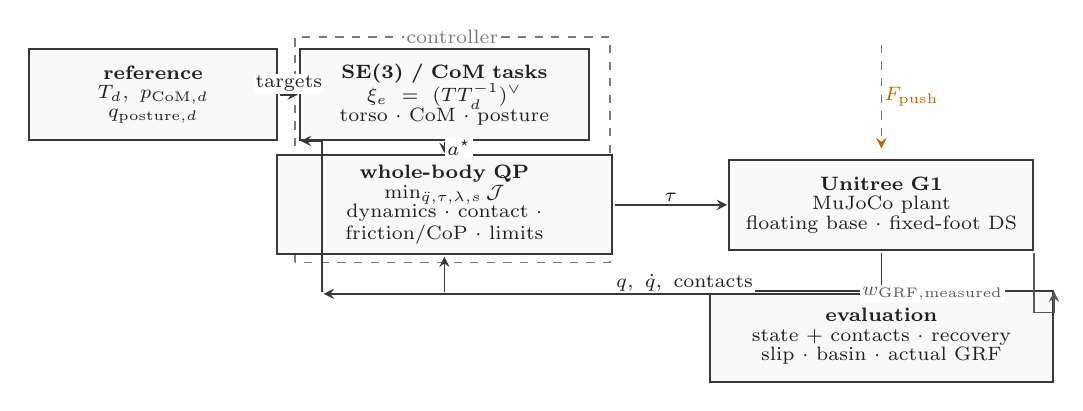
\begin{tikzpicture}[x=1cm,y=1cm]
    \ifdefined\CandidateSheet
      \node[anchor=west,font=\scriptsize,text=archmuted] at (-0.05,4.50)
        {Candidate B - controller boundary with external plant};
    \fi

    \draw[archboundary] (3.35,1.22) rectangle (7.35,4.08);
    \node[archboundarylabel] at (5.35,4.08) {controller};

    \node[archref] (bref) at (1.55,3.35) {\textbf{reference}\\[-1pt]
      {\scriptsize $T_d,\ p_{\mathrm{CoM},d}$}\\[-1pt]
      {\scriptsize $q_{\mathrm{posture},d}$}};
    \node[archtask] (btask) at (5.25,3.35) {\textbf{SE(3) / CoM tasks}\\[-1pt]
      $\xi_e=\Log(TT_d^{-1})^\vee$\\[-1pt]
      {\scriptsize torso $\cdot$ CoM $\cdot$ posture}};
    \node[archqp] (bqp) at (5.25,1.95) {\textbf{whole-body QP}\\[-1pt]
      $\min_{\ddot q,\tau,\lambda,s}\mathcal{J}$\\[-1pt]
      {\scriptsize dynamics $\cdot$ contact $\cdot$ friction/CoP $\cdot$ limits}};
    \node[archplant] (bplant) at (10.80,1.95) {\textbf{Unitree G1}\\[-1pt]
      MuJoCo plant\\[-1pt]
      {\scriptsize floating base $\cdot$ fixed-foot DS}};
    \node[archeval] (beval) at (10.80,0.28) {\textbf{evaluation}\\[-1pt]
      {\scriptsize state + contacts $\cdot$ recovery}\\[-1pt]
      {\scriptsize slip $\cdot$ basin $\cdot$ actual GRF}};

    \draw[archsignal] (bref.east) --
      node[archlabel,above] {targets}
      (btask.west);
    \draw[archsignal] (btask.south) -- node[archmathlabel,right] {$a^\star$} (bqp.north);
    \draw[archsignal] (bqp.east) -- node[archmathlabel,above] {$\tau$} (bplant.west);

    \draw[archpushsignal] (10.80,4.00) --
      node[archpushlabel,right] {$F_{\mathrm{push}}$} (10.80,2.65);

    % The left branch reaches the upper task without passing through the QP;
    % the central branch reaches the QP directly.
    \coordinate (bfb) at (10.80,0.82);
    \draw[archfeedback] (bplant.south) -- (bfb) -- (3.70,0.82);
    \draw[archfeedback] (3.70,0.82) |- (btask.south west);
    \draw[archfeedback] (5.25,0.82) -- (bqp.south);
    \node[archlabel,above] at (8.30,0.82) {$q,\ \dot q,\ \mathrm{contacts}$};

    \draw[archmeasurement] (bplant.south east) -- ++(0,-0.78) -|
      (beval.north east);
    \node[archmeasurelabel,above] at (11.45,0.70)
      {$w_{\mathrm{GRF,measured}}$};
  \end{tikzpicture}%
}

% Candidate C: compact two-row architecture.  The upper row is the control
% path; the lower row is a deliberately separate physical-data/evaluation bus.
\newcommand{\DrawArchitectureCandidateC}{%
  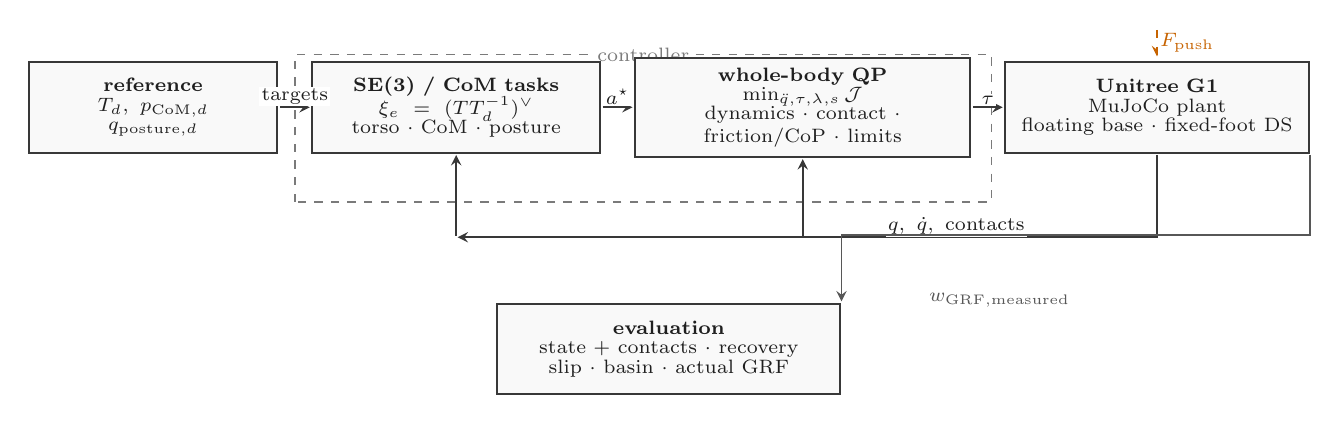
\begin{tikzpicture}[x=1cm,y=1cm]
    \ifdefined\CandidateSheet
      \node[anchor=west,font=\scriptsize,text=archmuted] at (-0.05,4.50)
        {Candidate C - compact two-row control and measurement bus};
    \fi

    \draw[archboundary] (3.35,2.15) rectangle (12.20,4.02);
    \node[archboundarylabel] at (7.775,4.02) {controller};

    \node[archref] (cref) at (1.55,3.35) {\textbf{reference}\\[-1pt]
      {\scriptsize $T_d,\ p_{\mathrm{CoM},d}$}\\[-1pt]
      {\scriptsize $q_{\mathrm{posture},d}$}};
    \node[archtask] (ctask) at (5.40,3.35) {\textbf{SE(3) / CoM tasks}\\[-1pt]
      $\xi_e=\Log(TT_d^{-1})^\vee$\\[-1pt]
      {\scriptsize torso $\cdot$ CoM $\cdot$ posture}};
    \node[archqp] (cqp) at (9.80,3.35) {\textbf{whole-body QP}\\[-1pt]
      $\min_{\ddot q,\tau,\lambda,s}\mathcal{J}$\\[-1pt]
      {\scriptsize dynamics $\cdot$ contact $\cdot$ friction/CoP $\cdot$ limits}};
    \node[archplant] (cplant) at (14.30,3.35) {\textbf{Unitree G1}\\[-1pt]
      MuJoCo plant\\[-1pt]
      {\scriptsize floating base $\cdot$ fixed-foot DS}};
    \node[archeval] (ceval) at (8.10,0.28) {\textbf{evaluation}\\[-1pt]
      {\scriptsize state + contacts $\cdot$ recovery}\\[-1pt]
      {\scriptsize slip $\cdot$ basin $\cdot$ actual GRF}};

    \draw[archsignal] (cref.east) --
      node[archlabel,above] {targets}
      (ctask.west);
    \draw[archsignal] (ctask.east) -- node[archmathlabel,above] {$a^\star$} (cqp.west);
    \draw[archsignal] (cqp.east) -- node[archmathlabel,above] {$\tau$} (cplant.west);

    \draw[archpushsignal] (14.30,4.35) --
      node[archpushlabel,right] {$F_{\mathrm{push}}$} (14.30,3.98);

    % Upper control row and lower physical-data row are separated by a clear
    % horizontal bus, which makes evaluation visibly external to the loop.
    \coordinate (cfb) at (14.30,1.70);
    \draw[archfeedback] (cplant.south) -- (cfb) -- (5.40,1.70);
    \draw[archfeedback] (5.40,1.70) -- (ctask.south);
    \draw[archfeedback] (9.80,1.70) -- (cqp.south);
    \node[archlabel,above] at (11.75,1.70) {$q,\ \dot q,\ \mathrm{contacts}$};

    \draw[archmeasurement] (cplant.south east) -- ++(0,-1.03) -|
      (ceval.north east);
    \node[archmeasurelabel,above] at (12.30,0.78)
      {$w_{\mathrm{GRF,measured}}$};
  \end{tikzpicture}%
}

% Final horizontal controls-paper layout. Desired quantities are signals
% rather than a separate subsystem; the plant and evaluation remain outside
% the dashed controller boundary.
\newcommand{\DrawArchitectureHorizontalFinal}{%
  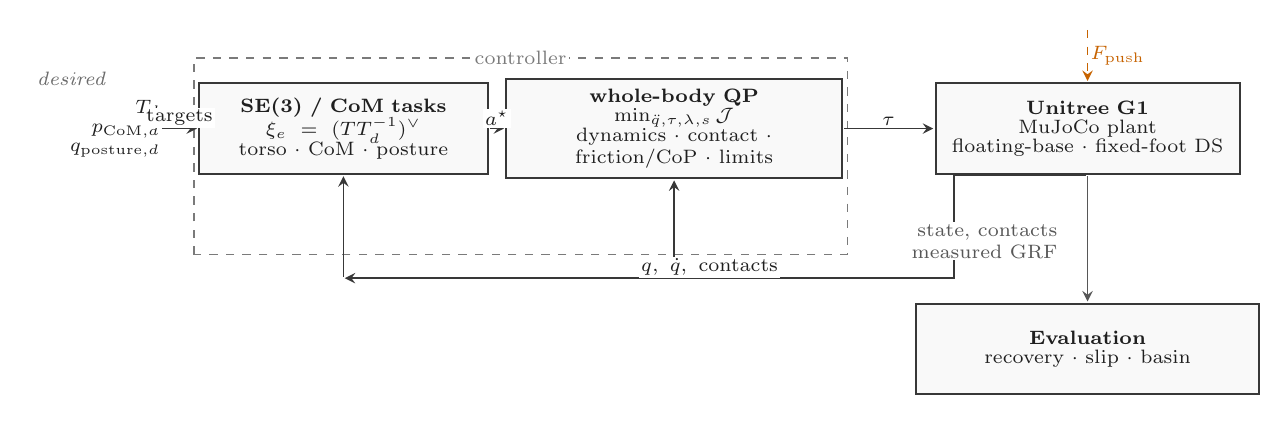
\begin{tikzpicture}[x=1cm,y=1cm]
    \draw[archboundary] (3.55,1.55) rectangle (11.85,4.05);
    \node[archboundarylabel] at (7.70,4.05) {controller};

    \node[archinput] (hdesired) at (2.55,3.15)
      {$T_d$\\[-1pt]$p_{\mathrm{CoM},d}$\\[-1pt]$q_{\mathrm{posture},d}$};
    \node[font=\scriptsize\itshape,text=archmuted,anchor=east]
      at (2.55,3.78) {desired};

    \node[archtask] (htask) at (5.45,3.15)
      {\textbf{SE(3) / CoM tasks}\\[-1pt]
      $\xi_e=\Log(TT_d^{-1})^\vee$\\[-1pt]
      {\scriptsize torso $\cdot$ CoM $\cdot$ posture}};
    \node[archqp] (hqp) at (9.65,3.15)
      {\textbf{whole-body QP}\\[-1pt]
      $\min_{\ddot q,\tau,\lambda,s}\mathcal{J}$\\[-1pt]
      {\scriptsize dynamics $\cdot$ contact $\cdot$ friction/CoP $\cdot$ limits}};
    \node[archplant] (hplant) at (14.90,3.15)
      {\textbf{Unitree G1}\\[-1pt]
      {\scriptsize MuJoCo plant}\\[-1pt]
      {\scriptsize floating-base $\cdot$ fixed-foot DS}};
    \node[archeval] (heval) at (14.90,0.35)
      {\textbf{Evaluation}\\[-1pt]
      {\scriptsize recovery $\cdot$ slip $\cdot$ basin}};

    \draw[archsignal] (hdesired.east) --
      node[archlabel,above] {targets}
      (htask.west);
    \draw[archsignal] (htask.east) --
      node[archmathlabel,above] {$a^\star$}
      (hqp.west);
    \draw[archsignal] (hqp.east) --
      node[archmathlabel,above] {$\tau$}
      (hplant.west);

    \draw[archpushsignal] (14.90,4.42) --
      node[archpushlabel,right] {$F_{\mathrm{push}}$}
      (hplant.north);

    % One bottom state bus feeds both controller blocks.
    \draw[archfeedback] (hplant.south) -- ++(-1.70,0) |- (5.45,1.25);
    \draw[archfeedback] (5.45,1.25) -- (htask.south);
    \draw[archfeedback] (9.65,1.25) -- (hqp.south);
    \node[archlabel,above] at (10.10,1.25)
      {$q,\ \dot q,\ \mathrm{contacts}$};

    % Direct physical measurement path to evaluation; no side U-turn.
    \draw[archmeasurement] (hplant.south) -- (heval.north);
    \node[archmeasurelabel,anchor=east,align=right] at (14.55,1.72)
      {state, contacts\\ measured GRF};
  \end{tikzpicture}%
}
